 \section{Behavioral Pattern}
In this section, the behavior of the two major classes \class{Problem} and \class{Person} are described. 
These two are the only classes which can have more states. 

\subsection{Problem}
\label{sub:problem}
Figure \ref{fig:Klasse_diagram_problem} shows the behavior of a problem. 
Note that you can solve the problem by attaching one or more solutions. 
A problem can have an unlimited number of solutions. 
You can at all times delete the problem, thus the arrow points from the edge of the box.
\begin{figure}[H]
\begin{center}
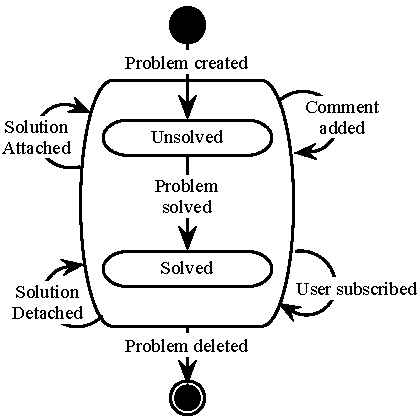
\includegraphics[scale=1]{input/problem_domain_analysis/Klassediagram_problem.pdf}
\morscaption{The statechart of the problem class}
\label{fig:Klasse_diagram_problem}
\end{center}
\end{figure}

\subsection{Person}
As shown in figure \ref{fig:Klasse_diagram_person}, a person is assigned a role in the application as soon as he is created. 
He can only have one role at a time. 
The roles inherit from each other. 
Meaning that a admin can do the same as the client, but clients can not do the same as admin. 
\begin{figure}[H]
\begin{center}
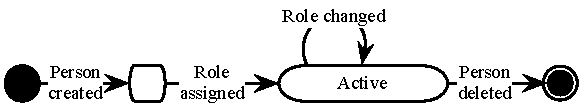
\includegraphics[scale=1]{input/problem_domain_analysis/Klassediagram_person.pdf}
\morscaption{The class person's statechart}
\label{fig:Klasse_diagram_person}
\end{center}
\end{figure}